%\chapter{Obsah CD}
%\chapter{Manual}
%\chapter{Konfigraèní soubor}
%\chapter{RelaxNG Schéma konfiguraèního soboru}
%\chapter{Plakat}
\chapter{AES Properties}
\begin{algorithm}
\caption{AES decryption}
\label{decr}
\begin{algorithmic}
\State \textbf{Decipher(State, Key)}
\State state $\gets AddRoundKey($State, Key[n]$)$
\State state $\gets ShiftRows($state$)$
\State state $\gets SubBytes($state$)$
\vspace{0.5em}
\For{$i \gets (n-1..1)$}
    \State state $\gets AddRoundKey($state, Key[i]$)$
    \State state $\gets MixColumns($state$)$
    \State state $\gets ShiftRows($state$)$
    \State state $\gets SubBytes($state$)$
\EndFor
\vspace{0.5em}
\State state $\gets AddRoundKey($state, Key[0]$)$
\vspace{0.5em}
\State $return$ state
\end{algorithmic}
\end{algorithm}

\begin{table}
\label{sbox}
\begin{center}
\begin{tabular}{|c|cccccccccccccccc|}\hline%
      &  0 &  1 &  2 &  3 &  4 &  5 &  6 &  7 &  8 &  9 &  a &  b &  c &  d &  e &  f \\\hline
   00 & 63 & 7c & 77 & 7b & f2 & 6b & 6f & c5 & 30 & 01 & 67 & 2b & fe & d7 & ab & 76 \\ 
   10 & ca & 82 & c9 & 7d & fa & 59 & 47 & f0 & ad & d4 & a2 & af & 9c & a4 & 72 & c0 \\ 
   20 & b7 & fd & 93 & 26 & 36 & 3f & f7 & cc & 34 & a5 & e5 & f1 & 71 & d8 & 31 & 15 \\ 
   30 & 04 & c7 & 23 & c3 & 18 & 96 & 05 & 9a & 07 & 12 & 80 & e2 & eb & 27 & b2 & 75 \\ 
   40 & 09 & 83 & 2c & 1a & 1b & 6e & 5a & a0 & 52 & 3b & d6 & b3 & 29 & e3 & 2f & 84 \\ 
   50 & 53 & d1 & 00 & ed & 20 & fc & b1 & 5b & 6a & cb & be & 39 & 4a & 4c & 58 & cf \\ 
   60 & d0 & ef & aa & fb & 43 & 4d & 33 & 85 & 45 & f9 & 02 & 7f & 50 & 3c & 9f & a8 \\ 
   70 & 51 & a3 & 40 & 8f & 92 & 9d & 38 & f5 & bc & b6 & da & 21 & 10 & ff & f3 & d2 \\ 
   80 & cd & 0c & 13 & ec & 5f & 97 & 44 & 17 & c4 & a7 & 7e & 3d & 64 & 5d & 19 & 73 \\ 
   90 & 60 & 81 & 4f & dc & 22 & 2a & 90 & 88 & 46 & ee & b8 & 14 & de & 5e & 0b & db \\ 
   a0 & e0 & 32 & 3a & 0a & 49 & 06 & 24 & 5c & c2 & d3 & ac & 62 & 91 & 95 & e4 & 79 \\ 
   b0 & e7 & c8 & 37 & 6d & 8d & d5 & 4e & a9 & 6c & 56 & f4 & ea & 65 & 7a & ae & 08 \\ 
   c0 & ba & 78 & 25 & 2e & 1c & a6 & b4 & c6 & e8 & dd & 74 & 1f & 4b & bd & 8b & 8a \\ 
   d0 & 70 & 3e & b5 & 66 & 48 & 03 & f6 & 0e & 61 & 35 & 57 & b9 & 86 & c1 & 1d & 9e \\ 
   e0 & e1 & f8 & 98 & 11 & 69 & d9 & 8e & 94 & 9b & 1e & 87 & e9 & ce & 55 & 28 & df \\ 
   f0 & 8c & a1 & 89 & 0d & bf & e6 & 42 & 68 & 41 & 99 & 2d & 0f & b0 & 54 & bb & 16 \\ 
\hline
\end{tabular}
\end{center}
\caption{S-box for SubBytes transformation in hexadecimal notation.}
\end{table}

\begin{table}
\label{invsbox}
\begin{center}
\begin{tabular}{|c|cccccccccccccccc|}\hline%
      &  0 &  1 &  2 &  3 &  4 &  5 &  6 &  7 &  8 &  9 &  a &  b &  c &  d &  e &  f \\\hline
   00 & 63 & 7c & 77 & 7b & f2 & 6b & 6f & c5 & 30 & 01 & 67 & 2b & fe & d7 & ab & 76 \\ 
   10 & ca & 82 & c9 & 7d & fa & 59 & 47 & f0 & ad & d4 & a2 & af & 9c & a4 & 72 & c0 \\ 
   20 & b7 & fd & 93 & 26 & 36 & 3f & f7 & cc & 34 & a5 & e5 & f1 & 71 & d8 & 31 & 15 \\ 
   30 & 04 & c7 & 23 & c3 & 18 & 96 & 05 & 9a & 07 & 12 & 80 & e2 & eb & 27 & b2 & 75 \\ 
   40 & 09 & 83 & 2c & 1a & 1b & 6e & 5a & a0 & 52 & 3b & d6 & b3 & 29 & e3 & 2f & 84 \\ 
   50 & 53 & d1 & 00 & ed & 20 & fc & b1 & 5b & 6a & cb & be & 39 & 4a & 4c & 58 & cf \\ 
   60 & d0 & ef & aa & fb & 43 & 4d & 33 & 85 & 45 & f9 & 02 & 7f & 50 & 3c & 9f & a8 \\ 
   70 & 51 & a3 & 40 & 8f & 92 & 9d & 38 & f5 & bc & b6 & da & 21 & 10 & ff & f3 & d2 \\ 
   80 & cd & 0c & 13 & ec & 5f & 97 & 44 & 17 & c4 & a7 & 7e & 3d & 64 & 5d & 19 & 73 \\ 
   90 & 60 & 81 & 4f & dc & 22 & 2a & 90 & 88 & 46 & ee & b8 & 14 & de & 5e & 0b & db \\ 
   a0 & e0 & 32 & 3a & 0a & 49 & 06 & 24 & 5c & c2 & d3 & ac & 62 & 91 & 95 & e4 & 79 \\ 
   b0 & e7 & c8 & 37 & 6d & 8d & d5 & 4e & a9 & 6c & 56 & f4 & ea & 65 & 7a & ae & 08 \\ 
   c0 & ba & 78 & 25 & 2e & 1c & a6 & b4 & c6 & e8 & dd & 74 & 1f & 4b & bd & 8b & 8a \\ 
   d0 & 70 & 3e & b5 & 66 & 48 & 03 & f6 & 0e & 61 & 35 & 57 & b9 & 86 & c1 & 1d & 9e \\ 
   e0 & e1 & f8 & 98 & 11 & 69 & d9 & 8e & 94 & 9b & 1e & 87 & e9 & ce & 55 & 28 & df \\ 
   f0 & 8c & a1 & 89 & 0d & bf & e6 & 42 & 68 & 41 & 99 & 2d & 0f & b0 & 54 & bb & 16 \\ 
\hline
\end{tabular}
\end{center}
\caption{Inverse S-box for SubBytes transformation in hexadecimal notation.}
\end{table}

\begin{figure}[H]
\centering
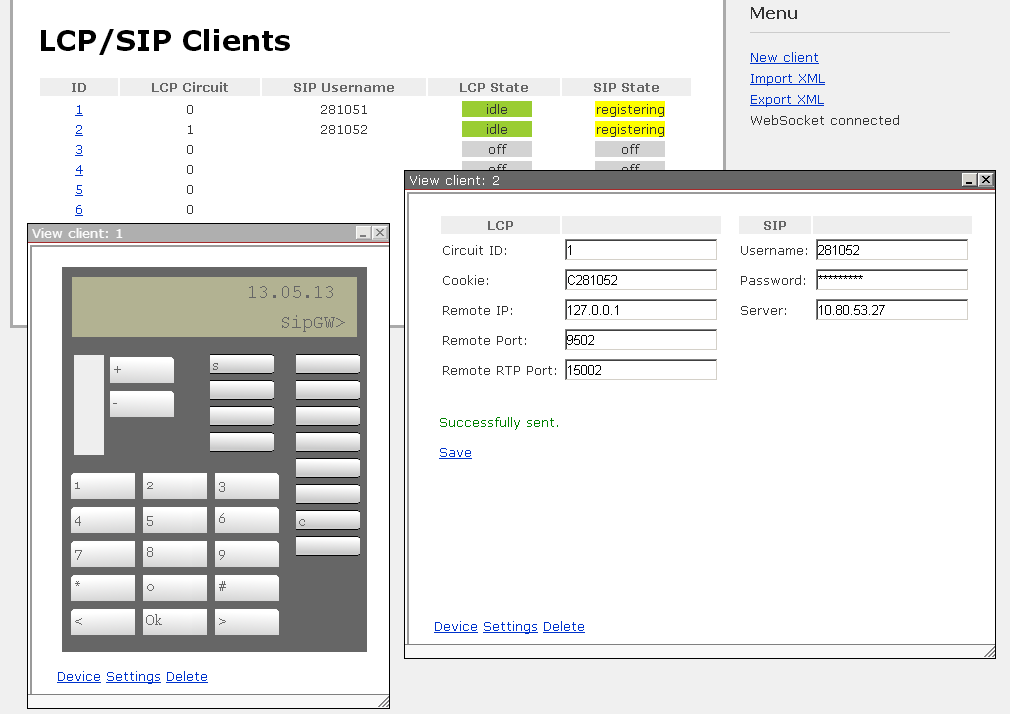
\includegraphics[width=15cm]{fig/screen.png}
\caption[Management tool screenshot]{Management tool screenshot.}
\label{pt_payload}
\end{figure} 
